\section{Процессы разработки}

\subsection{Сравнительный анализ методологий управления разработкой}

Для определения оптимального пути реализации проекта были рассмотрены три доминирующих парадигмы в индустрии программного обеспечения:
\begin{itemize}
    \item \textbf{Каскадная модель (Waterfall)}: Подход, при котором все требования обговариваются до начала работы. Несмотря на предсказуемость, метод был отвергнут, потому что была высокая степень неопределенности продукта. В разработке сайта нужно иметь возможность интерфейс на основе первых тестов, что невозможно в жестких рамках Waterfall.
    \item \textbf{Scrum-фреймворк~\cite{scrum-guide}}: Итеративный подход, который ориентирован на кросс-
    функциональность. 
    Команда отказалась от "чистого" Scrum, так как в условиях становления команды и наличия ярко выраженной специализации (выделенная роль аналитика) возникал риск неэффективного планирования и простоев разработчиков в ожидании документации в начале спринта.
    \item \textbf{Kanban-метод~\cite{kanban-book-and}}: Система управления потоком, минимизирующая незавершенное производство (WIP). Несмотря на использование элементов Kanban в самой тематике нашего продукта, для внутренней разработки метод показался недостаточно структурированным для новой команды, которой необходим спринты для поддержания темпа.
\end{itemize}

\subsection{Обоснование гибридного подхода: Асинхронный пайплайн}

В результате анализа был сформирован гибридный метод, сочетающий дисциплину Scrum (итерации) и принципы управления потоком. Суть метода заключается в разделении жизненного цикла задачи на два параллельных трека:

Аналитика: Опережающая работа аналитика. Пока команда разработки занята текущей итерацией, аналитик готовит документацию, схемы API и требования для следующей "Стори". Это позволяет нивелировать риск "пустого бэклога" на старте итерации.

Разработка: Реализация согласованного объема задач разработчиками в фиксированные циклы от 1 до 3 недель. Данная схема научно обоснована Теорией ограничений Э. Голдратта~\cite{gold-goal-book}. Выделяя аналитику в отдельный этап, мы расширяем "узкое горлышко" системы, обеспечивая максимальную пропускную способность команды разработки.

\begin{figure}[htbp]
    \centering
    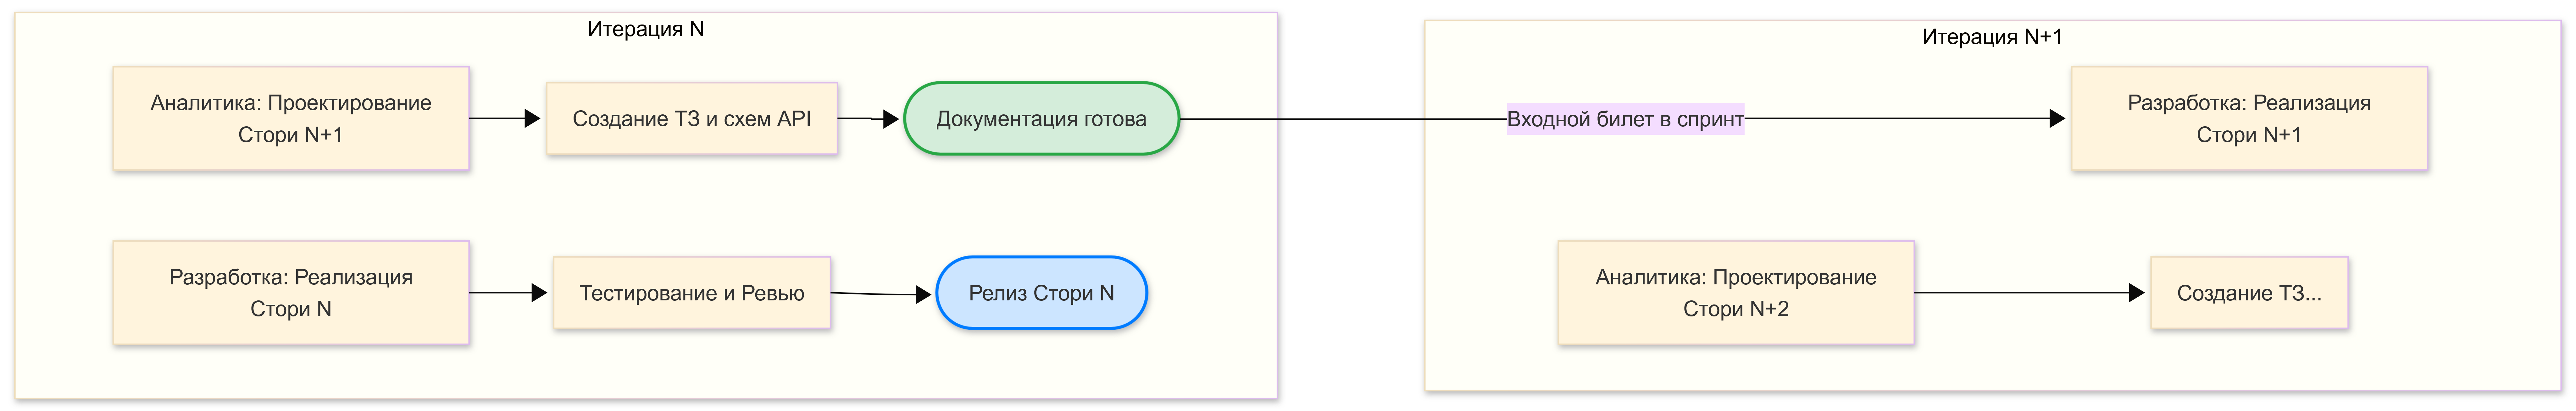
\includegraphics[width=0.95\textwidth]{../graphics/pipeline.png}
    \caption{Схема асинхронного пайплайна гибридного процесса разработки}
    \label{fig:async_pipeline}
\end{figure}

\newpage

\subsection{Жизненный цикл задачи} 
Работа над каждой стори в нашей команде делится на несколько последовательных шагов:

\begin{enumerate}
    \item \textbf{Аналитика}: Проработка ролевых моделей, построение схемы взаимодействия с API, продумывание дизайна при Front-end разработке. Здесь происходит декомпозиция стори с учетом процесса разработки.
    \item \textbf{Встреча 3-Amigos}: Короткий созвон, на которой аналитик (один из разработчков по очередности) презентует документацию. На этом этапе планируется работа и распределяются задачи между Front-end, Back-end и DevOps. Это позволяет прояснить все вопросы до старта разработки.
    \item \textbf{Реализация}: Разработка, покрытие юнит-тестами и настройка мониторинга/аллертов.
\end{enumerate} 

Подобное разделение опирается на "Lean Thinking"~\cite{lean-book}. Это позволяет не терять время на выяснение деталей и снижает количество ошибок в требованиях.

\subsection{Визуализация и контроль потока} 
Чтобы наглядно контролировать разработку, в проекте используется электронная канбан-доска. Она построена под наш гибкий метод и показывает, как каждая задача проходит четыре этапа:

\begin{enumerate}
    \item \textbf{Todo:} этап формирования и приоритезации бэклога.
    \item \textbf{In progress:} активная фаза реализации. Для задач аналитики этот этап подразумевает исследование и создание документации. Для задач разработки - написание кода на основе уже готовых требований.
    \item \textbf{Review:}  этап верификации. В контексте аналитики этот статус означает проведение встречи, на которой аналитик представляет свое решение. В контексте разработки - проведение код-ревью и контроль качества.
    \item \textbf{Done:} задача проверена, соответствует критериям качества и идет в релиз.
\end{enumerate}

Особое внимание уделяется правилам перехода между этапами. Разработчики берут стори в работу только после полного завершения аналитики. Это исключает старт разработки по сырым требованиям и поддерживает ровный поток задач. Именно такой подход диктуют закон Литтла~\cite{little-law} и теория ограничений~\cite{gold-goal-book}.

Все процессы были рассматрены и утверждены командой в качестве стандартов коммуникации.

\begin{figure}[htbp]
    \centering
    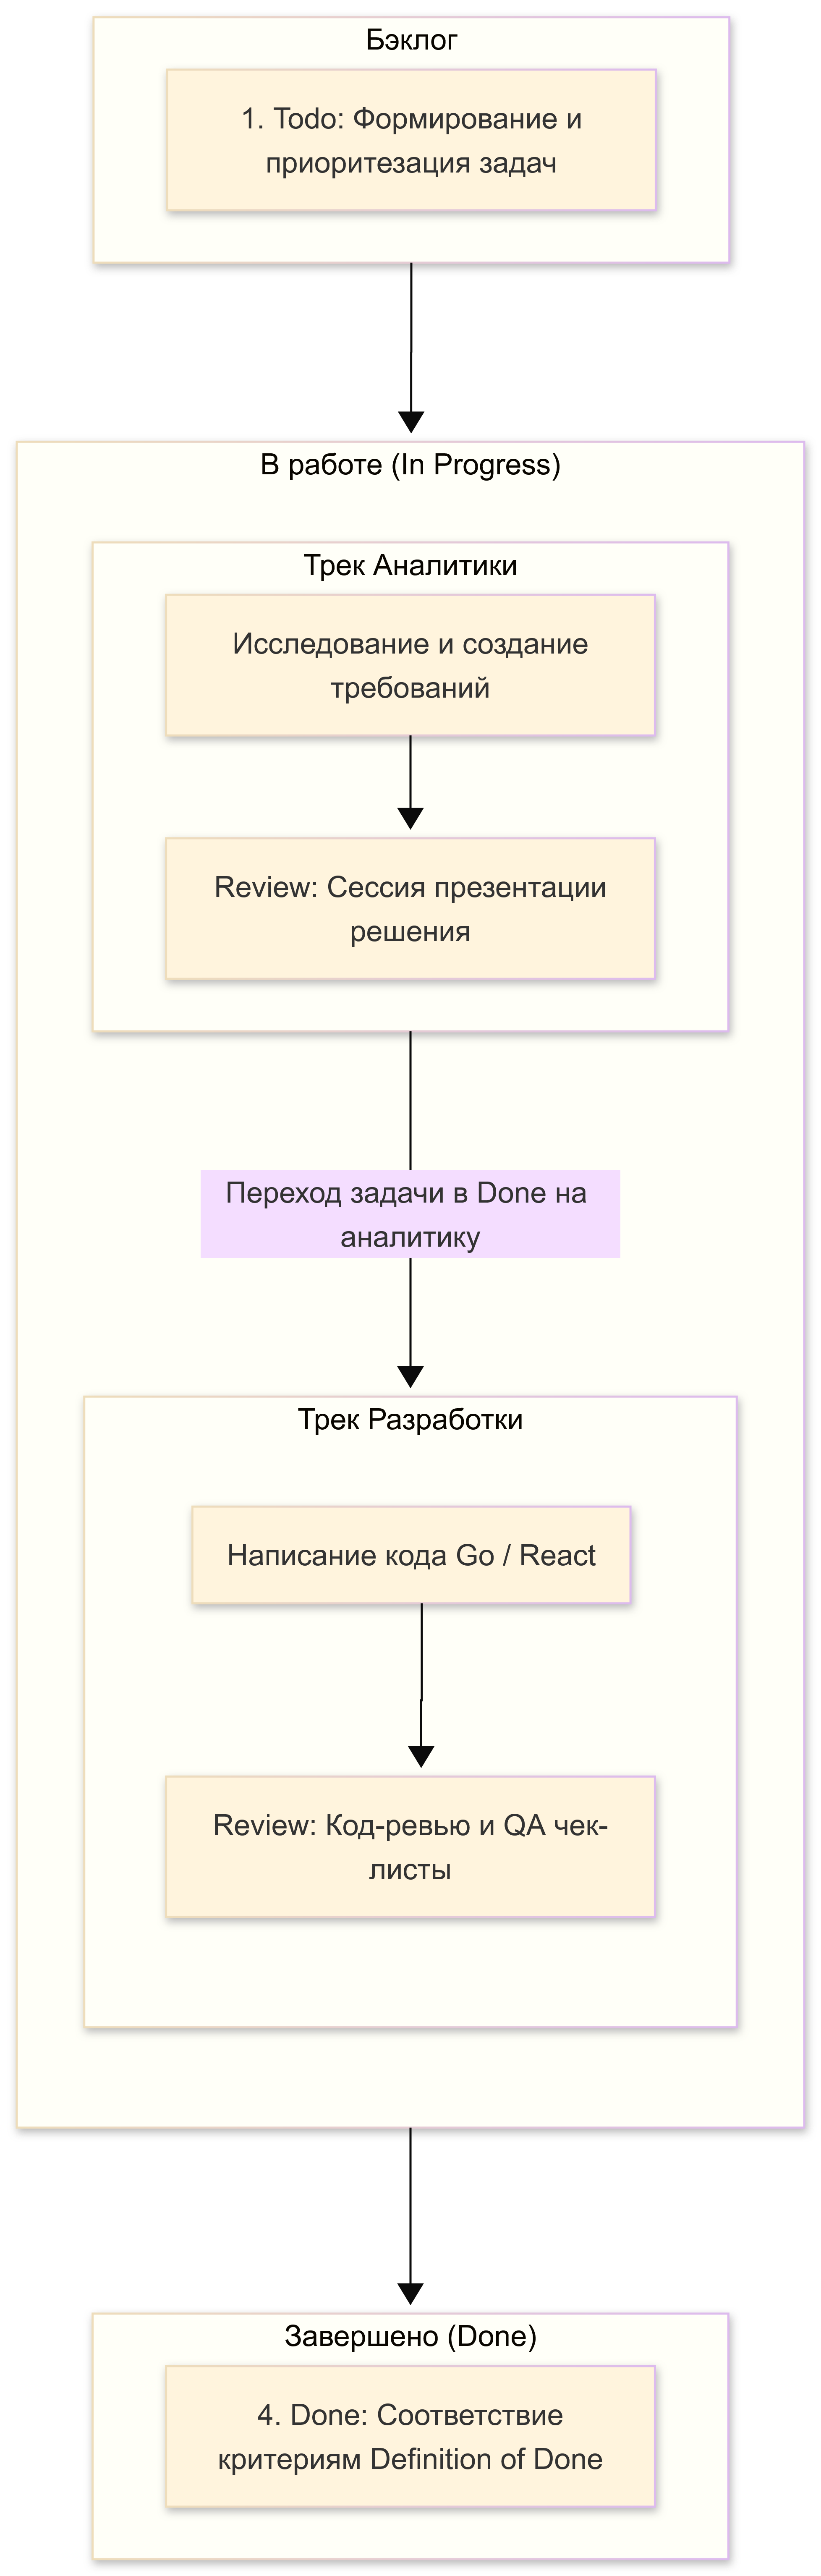
\includegraphics[height=0.8\textwidth]{../graphics/kanban_flow.png}
    \caption{Этапы прохождения функциональной единицы (Стори) по Канбан-доске}
    \label{fig:kanban_flow}
\end{figure}